%!TEX root = New.tex

\section{Trace-driven evaluation}
%TBD: terminology regular name, mobile names, highly mobile and low mobile names
%TBD: write a table and put all statistics in the table, refer the SoftRate paper
%TBD: don't show UNIFORM everywhere, just show UNIFORM in one place, say this is how much locality improve, then just show locality
%TBD: STATIC K? why 3, need an experiment that changes K
%TBD: replace "why" in bullet with the actual reason, what is scalability?(three things)
%TBD: straight lines for REPLICATEALL and CoDoNS odd, more interpolation
%TBD: Figure 17, another LOCALITY that is much worse than LOCALITY
%TBD: write the scheme description, what is load-awareness: replication side and client side
%TBD: just four graphs, simulator validation, load, number of name servers, ratio of mobile to regular names, number of total names, ratio of aggregate reads for regular and mobile, locality of mobile names, top-K


\begin{table*}[t]
\centering
\small{
\begin{tabular}{c|c|c|c|c}
{\bf Section} & {\bf Evaluation method} & {\bf \# names} & {\bf \# servers} & {\bf load (req/sec)} \\ \hline
\S \ref{sim:load} & Trace-driven, varying load & 10K regular, 100K mobile & 10K & 10 to 100K \\ \hline
\S \ref{sim:numns} & Trace-driven, varying \# servers & 10K regular, 100K mobile &  100 to 100K & 1K \\ \hline
\S \ref{sim:numname} & Trace-driven, varying \# names & 10K regular, 1K to 1M mobile & 10K & 10K\\ \hline
\end{tabular}
}
\end{table*}


\bp{why trace-driven evaluation}
Due to the limitation in flexibility and scalability of the planetlab platform, in this section, we further conduct trace-driven experiments to evaluate \auspice\ under a variety of scalability scenarios. Our evaluation shows that \auspice\ scales well and improves user-perceived latency by TDB$\times$ at growing system load (\S TBD), growing number of name servers (\S TBD) and growing number of name services (\S TBD).
 
\subsection{Experimental setup}

\subsubsection{Dataset}
\label{subsubsec:dataset}

We used data from Alexa Web Information Service  (AWIS)  \cite{alexa} as the basis of our name service dataset. AWIS provides traffic statistics for websites collected via web crawls and web usage reported by Alexa Toolbar users.
We have collected (after paying a nominal fee) two types of traffic data for the top 100,000 websites from AWIS:  
(1) Page views percent (PgViewPct): the fraction of a website's page views out of all the page views in the Internet;
(2) City page views percent (CityPgViewPct): the fraction of a city's page views for a website out of all the page views for this website, i.e., a website's page view percent breakdown by cities.
\footnote{CityPgViewPct is unavailable for TBD-TBD\% of page views for different websites.
We normalize the fraction of page views from each city so that the aggregate page views fractions of all cities sums up to one.} 

\subsubsection{Workload}

\bp{name service workload}
Our name service workload consists of a sequence of requests  of name record of websites by users and updates to the name record by the website owner.
Each service is a naming service for a unique domain name, and each user-group consists of all users from the same city.
Domain names are categorized into regular names and mobile names, which have different workloads respectively.

\bp{workload for regular names}
The workload for regular names are generated using the AWIS dataset (refer \S \ref{subsubsec:dataset}). For each website, the total number of requests for its name record is proportional to its PgViewPct, and the number of requests from each city is proportional to the PgViewPct $\times$ CityPgViewPct.
AWIS does not report the frequency at which name records are updated for each website.
We assume that each name record has a fixed update rate equal to a random value in the range of 0.01$\times$ to 0.1$\times$ of the request rate for the name.  As a result, regular names have request rates between TBD and TBD requests per day and update rates between TBD and TBD updates per day.
We use a default TTL of 0 for regular names in most experiments and we evaluate the effect of TTL in \S TBD.

\bp{workload for mobile names}
Mobile names can have dramatic different workload from regular names because of their highly mobility and locality nature. In our workloads, we assume each mobile name has a request rate uniformly distributed between 1 and 10 requests per day and an update rate uniformly distributed between 10 and 100 updates per day. Requests for a mobile name is generated from five geographically closest cities. Mobile names don't have a TTL value so all requests go to the name servers directly.

\bp{aggregate experiment statistics}
In all our experiments we generate workloads for 10K regular names and 100K mobile names except in \S TBD where we increase the number of mobile names to evaluate the scalability of \auspice. In each run of the experiment, we generate 10 million name record requests, out of which 90\% are for regular names and 10\% are for mobile names; and we generate 9 million updates,  out of which 5\% are for regular names and 95\% are for mobile names.

\subsubsection{Compared replication algorithms}

We compare \auspice\ against the following service replication algorithms:

{\it STATIC3}, which places each name service at a static number three of replicas. The three replicas are chosen through three hash functions so as to optimize for load balancing. 

{\it CoDoNS} \cite{codons}, which places name services through a DHT peer-to-peer overlay so as to optimize the total number of replicas.

{\it UNIFORM},  which uses the same scheme (Eq. \ref{}) as \auspice\ to determine the number of replicas, but unlike the voting scheme of \auspice\ it select replicas randomly.

{\it REPLICATEALL}, which places each name service at all name servers.

{\it OPTIMAL}, 

These four alternative algorithms represent reasonable approaches to optimize different system metrics ---- while STATIC3 and REPLICATEALL optimize load and latency respectively in a naive way, CoDoNS and UNIFORM try to optimize one metric without hurting the other in a more sophisticated manner.

\subsection{Trace-driven simulator validation}
\label{subsec:simulatorval}

\bp{How we do simulator validation}
Our evaluation of \auspice\ in later sections is based on a trace-driven simulator. The simulator takes as input a list of geographical locations for local name servers and name servers, their ping latencies, a sequence of name service request and update, and a replication algorithm. We validate our simulator by feeding the above trace from the Planetlab deployment to the simulator and comparing the simulation result against the deployment result. We also noticed that each Planetlab node has an almost constant non-zero processing latency because of the load on it, thus we add that latency value on top of the ping latency as the final latency for a request or update. The numbers of name services are 1K for regular and 10K for mobile in order to be consistent with the deployment, but all our later experiments use 10K regular names and 100K mobile names.

\bp{validation result}
Figure \ref{fig:simulatorval} shows the average request latency across names for the Planetlab deployment and the simulator. The errorbar shows the 5th and 95th percentile values. We've further verified that the latency difference between the simulation and the deployment is within 8\% at all the 100 percentiles, which validates the accuracy of our simulator.

\begin{figure}[t]
\centering
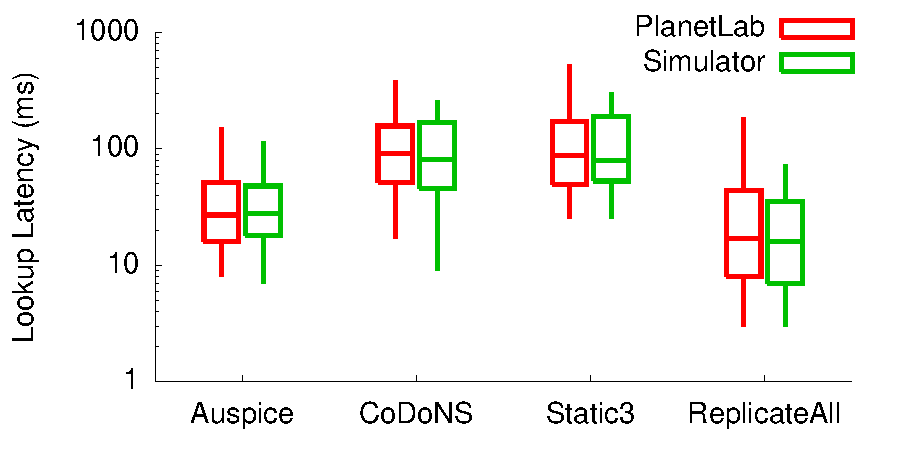
\includegraphics[scale=0.5]{graph/simulatorval1.pdf}
\caption{Average request latency across names on Planetlab compared to trace-driven simulator. Boxplot shows 5th, Q1, median, Q3, 95th.}
\label{fig:simulatorval}
\end{figure}


\subsection{Varying load}
\label{sim:load}

\bp{Experimental setup for load experiment}
In this subsection, we evaluate \auspice\ under changing load. The experimental setup is similar to that in \S \ref{subsec:simulatorval}, i.e., we feed the name server locations and ping latencies from the Planetlab deployment to the simulator. In addition, we also specify a capacity and a synthetic load-induced latency model at each name server, which are unclear for the Planetlab nodes. We specify that each name server has a capacity of 10M request/update per day, i.e., each name server can process name record requests and updates at a rate no more than 10 million per day. We use M/M/1 queueing model \cite{mm1} to estimate  load-induced latency D:
$$D = \frac{\delta}{1- L/C}$$
where L is the load and C is the capacity at a name server, $\delta$ is a constant value (2.5 in our experiment). Thus latency for a request or update is the sum of ping latency between a local name server and a name server and the load-induced latency at the corresponding name server. When we vary the load, we vary both request and update rate at the same rate.

\bp{Figure  \ref{fig:meanlatencyvsload}: \auspice\ has best latency and scales well to load}
Figure \ref{fig:meanlatencyvsload} shows the average latency across names for different replication algorithms as the system load increases to a value where all algorithms start to have infinite latency. Each dot in the figure is the average value of the mean latency for all names, where mean latency for a name is the mean latency of all requests for a name.
Two conclusions can be drawn from the figure.
First, \auspice\ achieves the best latency performance, e.g., it improves latency by up to 4$\times$ over UNIFORM, the second best  algorithm and the one that places replicas randomly. This indicates that the voting scheme effectively places service replicas close to pockets of demands. 
Second, \auspice\ scales well at growing load. When the load is greater than 1500 req/sec, \auspice\ performs as well as (or even better than) STATIC3, a replication algorithm that incurs the least amount of update load. This is because \auspice\ is able to dynamically reduce the number of replicas (Eq. TBD) for each name service when it observes a high network load.

\bp{CoDoNS and REPLICATEALL have poor latency and  fail to scale to load}
In comparison, CoDoNS and REPLICATEALL have poor latency performance and fail to scale to load. 
CoDoNS has the highest latency because its DHT routing overlay fails to place replicas close to pockets of demands and routes request to the closest name server. Its latency starts to go infinite when load is greater than 1500 req/sec because it doesn't have a mechanism to adapt number of replicas at varying load. 
Likewise, REPLICATEALL incurs the highest update load and doesn't reduce its number of replicas, thus it fails to scale to load. (TBD: shall we omit its results for later experiments?)


\begin{figure}[t]
\centering
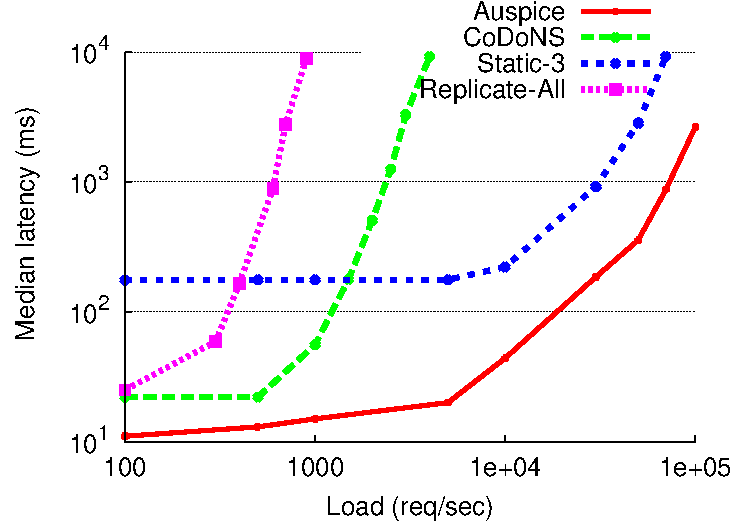
\includegraphics[scale=0.5]{graph/medianlatencyVSload.pdf}
\caption{[Varying load] Median latency across names under varying load. \auspice\ improves latency by up to TBD.}
\label{fig:meanlatencyvsload}
\end{figure}
Number of names: 10K regular, 100K mobile
Number of name servers: 10K
Number of local name servers: 1840?
NScapacity: 1M req/day
Number of request: 10M
total readrate 598877.56 regular fraction 0.90042746 mobile fraction 0.10004749
total writerate 583781.0 regular fraction 0.0506177 mobile fraction 0.9493815
avg hop count between 0.25 and 2.0


\subsection{Varying \# name servers}
\label{sim:numns}

Figure \ref{fig:numberNS}: latency VS \# name servers

\begin{figure}[t]
\centering
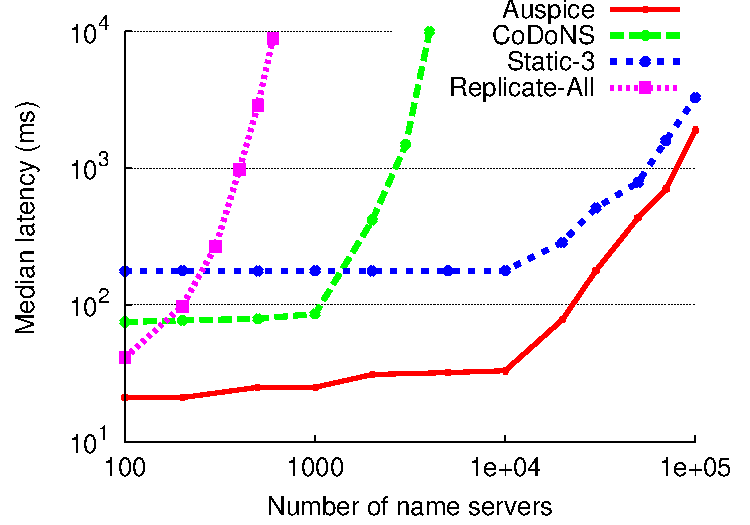
\includegraphics[scale=0.5]{graph/medianlatencyVSnumns.pdf}
\caption{[Varying \# servers] Median latency as \# name servers increases}
\label{fig:numberNS}
\end{figure}

Number of names: 10K regular, 100K mobile
Number of name servers: from 100 to 100K
Number of local name servers: 1840?
NScapacity: total is 10**10 req/day
Number of request: 10M
total readrate 598877.56 regular fraction 0.90042746 mobile fraction 0.10004749
total writerate 583781.0 regular fraction 0.0506177 mobile fraction 0.9493815
avg hop count between 0.25 and 2.0
at load 20 

\subsection{Varying \# names}
\label{sim:numname}

Figure \ref{fig:percentmobile}: latency VS \% mobile names
load 200

Number of read requests: 

Number of write requests:

Number of LNS(clients): 12,844

Number of name servers: 1000 (vary in Figure \ref{fig:numberNS} )

Number of regular names: 10,000

Number of mobile names: 100,000 (vary in Figure \ref{fig:percentmobile})

%Figure TBD: latency VS utilization threshold

%Figure TBD: latency VS mobile name locality 

%Figure TBD: latency VS TTL

\begin{figure}[t]
\centering
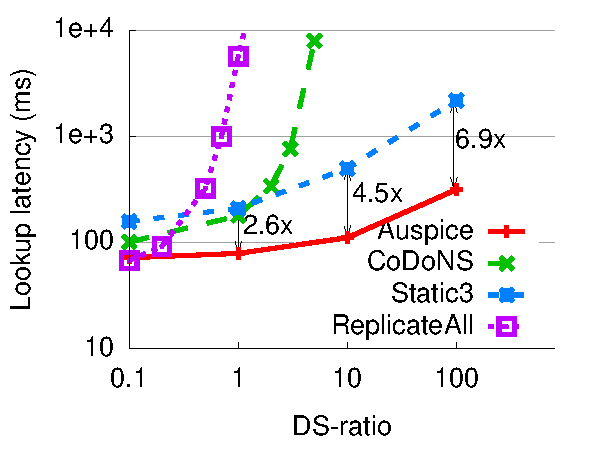
\includegraphics[scale=0.5]{graph/medianlatencyVSnummobile.pdf}
\caption{[Varying \# names] Median latency as percentage of mobile names increases}
\label{fig:percentmobile}
\end{figure}

\subsection{Comparison with OPTIMAL}

Figure \ref{fig:optimal}

\begin{figure}[t]
\centering
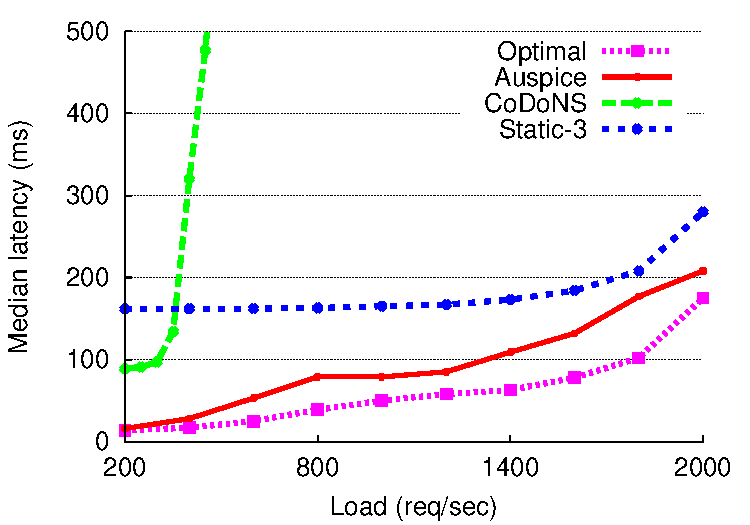
\includegraphics[scale=0.5]{graph/medianlatencyVSload_optimal.pdf}
\caption{Comparison with OPTIMAL}
\label{fig:optimal}
\end{figure}

%\bp{Figure \ref{fig:latencycdf}: \auspice\ improves latency across all names}
%Figure \ref{fig:latencycdf} further zooms into the latency CDF across names at a single load value of 150 request per second. Each dot in the figure is the mean latency of all requests for a name. \auspice\ improves latency across all names, and the median latency improvement over UNIFORM is  about 3$\times$.

%\bp{Figure \ref{fig:lossratevsload}: \auspice\ has lowest lossrate}
%Figure \ref{fig:lossratevsload} shows the average lossrate across names as load increases. \auspice\ has zero lossrate at low to moderate load and the lowest lossrate at high load. This again demonstrates the benefit of it being able to adapt the number of replicas to system load. In comparison, CoDoNS and REPLICATEALL fail to adapt to load and have lossrates growing to 100\% quickly when load increases. We notice that \auspice\ has significant lower lossrate than STATIC3 and UNIFORM when the latter two have lossrates close to 100\% at very high load. This is because STATIC3 and UNIFORM place replicas randomly and thus cause all name servers to be equally highly-loaded and drop all requests. However, \auspice\ places replicas close to demands of individual services and thus induces moderate load on some name servers that has fewer service demands. These name servers are able to respond to a large fraction of requests and thus making \auspice\ has lower lossrate.



%\subsubsection{Update cost}

%\bp{\auspice\ has update cost as low as STATIC3}
%Figure \ref{fig:updatecost} shows the update cost of different replication algorithms as load increases. The update cost is computed as the sum of the product of update rate and number of replicas for all name services. We use a single curve for \auspice\ and UNIFORM because they make the same number of replicas for each service and thus have the same update cost. Figure \ref{fig:updatecost} shows that \auspice\ has much lower update cost than CoDoNS and REPLICATEALL and has update cost as low as STATIC3 at high load. CoDoNS doesn't adapt its number of replicas thus has higher update cost when load increases. REPLICATEALL has the highest update cost because it replicates services at all name servers.


%\subsubsection{Load balance}
 
%Figure \ref{fig:fairness} shows the load balance performance for different algorithms. We measure this metric by computing Jain's fairness index \cite{}. When there are $n$ name servers with load $x_1$ through $x_n$, it is computed as 
%$$\frac{(\sum_{i=1}^n x_i )^2}{n \cdot  \sum_{i=1}^n x_i^2}$$
%\auspice\ has fair index comparable to the other algorithms at low load and has slightly worse fairness at high load. We note that \auspice\ sacrifices fairness for latency and lossrate (as shown in Figure \ref{fig:meanlatencyvsload} and \ref{fig:lossratevsload}).


%\subsubsection{Breakdown by names}

%\bp{Why breakdown by names}
%\auspice\ is designed for both regular and mobile name services that exhibit dramatic different request and update characteristics, i.e., the former has much more requests than updates and the latter vice versa. In this subsection, we evaluate \auspice's performance benefits  for these two types of name services respectively.

%{\bf Regular names}:
%Figure \ref{fig:meanlatencyvsload_regular} shows the average latency across regular names under varying load. \auspice\ outperforms the other replication algorithms and has slight better performance than UNIFORM. To explain this, we further look into the number of replicas it creates for each name service. Figure \ref{fig:numactives_regular} shows the average number of replicas across regular names. It shows that at low to moderate load, both \auspice\ and UNIFORM make a large number of replicas in order to fully utilize network capacity and optimize latency. It is not surprising that \auspice\ can't outperform UNIFORM with a large fraction of replicas. 


%{\bf Mobile names}:
%Figure \ref{fig:meanlatencyvsload_mobile} shows the average latency across mobile names. \auspice\ has significant latency improvement over UNIFORM. Figure \ref{fig:numactives_mobile} plots the average number of replicas across mobile names. It shows that \auspice\ (and UNIFORM) make use only a small fraction of name servers as replicas for each mobile name, therefore, the benefit's of \auspice\ placing replicas according to the locality of demands is significant.

